%-------------------------------------------------------------------------
% fonctions.tex
%-------------------------------------------------------------------------

%-------------------------------------------------------------------------
\setjobnamebeamerversion{fonctionsSlide}

\usetheme{Enib}
%-------------------------------------------------------------------------

%-------------------------------------------------------------------------
\newtheorem{rem}{Remarque}[section]
\newtheorem{defin}{Définition}[section]
\newtheorem{td}{\color{blue}TD}[section]
%-------------------------------------------------------------------------

%-------------------------------------------------------------------------
\lstset
{
language=Python,
basicstyle=\ttfamily,
identifierstyle=\ttfamily,
keywordstyle=\color{blue}\ttfamily,
commentstyle=\color{gray}\ttfamily,
stringstyle=\color{green}\ttfamily,
showstringspaces=false,
extendedchars=true,
numbers=left, 
numberstyle=\tiny,
frame=lines,
linewidth=0.95\textwidth,
xleftmargin=5mm
} 
%-------------------------------------------------------------------------

%-------------------------------------------------------------------------
\def\exo#1{\mbox{}\ \hfill\mbox{\color{blue}$\rule{2mm}{2mm}\,$\footnotesize\sc TD\ref{#1}}}
\def\exercice#1#2{\mbox{}\ \ TD \ref{#1}\ #2\ \dotfill\ \pageref{#1}\mbox{}}

\newenvironment{py}[1]{\begin{minipage}[t]{#1}\footnotesize}{\end{minipage}}
%-------------------------------------------------------------------------

\graphicspath{{../../fig/}}

%-------------------------------------------------------------------------
\title[Algorithmique]{\bf Initiation à l'algorithmique}
\subtitle{\bf --- procédures et fonctions ---\newline
1. Spécification et implémentation}


\author[\tt jacques.tisseau@enib.fr]{\large\bf Jacques TISSEAU}
\institute[\enib]{{\large\enib--\cerv}}
\date[enib\copyright 2009-2014]{\footnotesize enib\copyright 2009-2014}
%-------------------------------------------------------------------------

%-------------------------------------------------------------------------
\begin{document}
%-------------------------------------------------------------------------

%------------------------------------------
\begin{frame}<presentation>[label=titre]
\frametitle{Informatique \hfill {S1}}
%------------------------------------------
\titlepage

\end{frame}
\note{
\mbox{}\null\vfill

\begin{rem}[Notes de cours : couverture]
Ce support de cours accompagne le 
chapitre 3 des notes de cours « Initiation à l'algorithmique ».
$$\fbox{
\includegraphics[width=10cm,page=1]{../info-S1.pdf}}$$
\end{rem}
}
%------------------------------------------


%------------------------------------------
\begin{frame}<presentation>
\frametitle{Réutilisabilité des algorithmes}
%------------------------------------------
\begin{block}{Problème}
Comment réutiliser un algorithme existant sans avoir à le réécrire?
\end{block}
\pause

\begin{columns}[T]
\column{5cm}\footnotesize\tt
>>> n = 3\\
>>> f = 1\\
>>> for i in range(1,n+1):\\
...\ \ \ \ \ f = f*i\\
...\\
>>> f\\
6
\pause
\column{5cm}\footnotesize\tt
>>> n = 5\\
>>> f = 1\\
>>> for i in range(1,n+1):\\
...\ \ \ \ \ f = f*i\\
...\\
>>> f\\
120
\end{columns}
\pause
\begin{block}{Elément de réponse}
Encapsuler le code dans des fonctions ou des procédures.
\end{block}
\pause
\begin{columns}[T]
\column{5cm}\footnotesize\tt
>>> \alert{factorielle(}3\alert{)}\\
6
\pause
\column{5cm}\footnotesize\tt
>>> \alert{factorielle(}5\alert{)}\\
120
\end{columns}

\end{frame}
\note{
{\bf Définitions}\begin{description}
\item[réutilisabilité] aptitude d'un algorithme à
	être réutilisé pour résoudre des tâches équivalentes
	à celle pour laquelle il a été conçu.
\end{description}
}
%------------------------------------------


%------------------------------------------
\begin{frame}<presentation>
\frametitle{Structuration des algorithmes}
%------------------------------------------
\begin{block}{Problème}
Comment structurer un algorithme pour le rendre plus compréhensible ?
\end{block}
\pause
\begin{columns}[T]
\column{5.5cm}\tiny\tt
    ieee\_code = []\\
    k\_exponent = 8\\
    k\_significand = 23\\
    k\_ieee = 32\\
    bias = code(127,2,k\_exponent)\\
    x\_int = int(abs(x))\\
    x\_frac = abs(x) - x\_int\\
    expo\_2 = 0\\
    for i in range(k\_ieee): append(ieee\_code,0)\\
\mbox{}\\
    \# calcul du signe\\
    sign = int(x < 0)\\
\mbox{}\\ 
    \# calcul de la mantisse\\
    i = 0\\
    significand = []\\
    while (x\_int != 0) and (i < k\_significand):\\
\ \ \ \ insert(significand,0,x\_int\%2)\\
\ \ \ \ x\_int = x\_int/2\\
\ \ \ \ i = i + 1
\column{5.5cm}\tiny\tt
    if len(significand) > 0 and significand[0] == 1:\\
\ \ \ \ del significand[0]\\
\ \ \ \ expo\_2 = len(significand)\\
    i = len(significand)\\
    while (x\_frac != 0) and (i < k\_significand):\\
\ \ \ \ x\_frac = x\_frac * 2\\
\ \ \ \ x\_int = int(x\_frac)\\
\ \ \ \ x\_frac = x\_frac - x\_int\\
\ \ \ \ if (x\_int == 0) and (i == 0):\\
\ \ \ \ \ \ \ \ expo\_2 = expo\_2 - 1\\
        else:\\
\ \ \ \ \ \ \ \ append(significand,x\_int)\\
\ \ \ \ \ \ \ \ i = i + 1\\
\mbox{}\\
\pause
\alert{\em et quelques 20 lignes plus loin\ldots}\\
\mbox{}\\
\ \ \ \ ieee\_code[0] = sign\\
\ \ \ \ ieee\_code[1:9] = exponent\\
\ \ \ \ ieee\_code[9:32] = significand	    
\end{columns}
\end{frame}
\note{}
%------------------------------------------

%------------------------------------------
\begin{frame}<presentation>
\frametitle{Structuration des algorithmes}
%------------------------------------------
\begin{block}{Elément de réponse}
Utiliser des fonctions et des procédures.
\end{block}
\pause

$$\begin{minipage}{8cm}\footnotesize\tt
\# calcul du signe\\
sign = int(x < 0)\\
\mbox{}\\ 
\# calcul de la mantisse\\
significand, expo\_2 = \alert{mantisse(}x\alert{)}\\
\mbox{}\\ 
\# calcul de l'exposant\\
exponent = \alert{exposant(}expo\_2,127\alert{)}\\
\mbox{}\\
\# code IEEE 754\\
ieee\_code[0] = sign\\
ieee\_code[1:9] = exponent\\
ieee\_code[9:32] = significand
\end{minipage}$$
    
\end{frame}
\note{
{\bf Définitions}\begin{description}
\item[encapsulation] action de mettre une chose dans une autre
\end{description}
}
%------------------------------------------

%------------------------------------------
\begin{frame}<presentation>
\frametitle{Diviser pour régner}
%------------------------------------------
\begin{block}{Structuration}
Les fonctions et les procédures permettent de décomposer un programme complexe en une 
série de sous-programmes plus simples, lesquels peuvent à leur tour être décomposés 
eux-mêmes en fragments plus petits, et ainsi de suite.  
\end{block}
\pause

\centerline{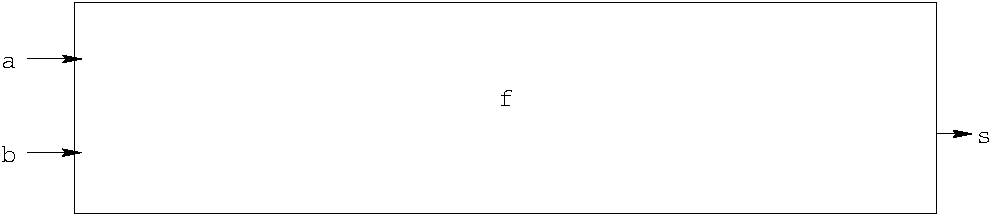
\includegraphics[width=8cm]{../fig/structure1.pdf}}
\pause 

\centerline{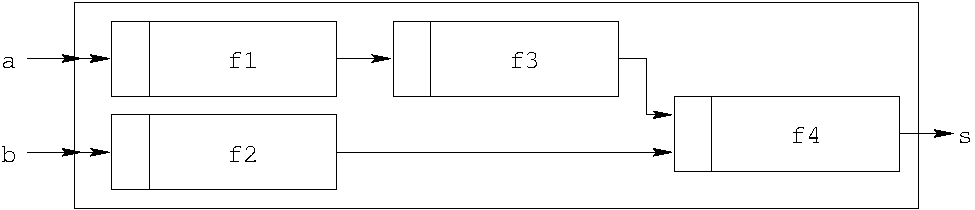
\includegraphics[width=8cm]{../fig/structure2.pdf}}

\end{frame}
\note{} 
%------------------------------------------


%------------------------------------------
\begin{frame}<presentation>
\frametitle{Fonctions}
%------------------------------------------
\begin{block}{Fonctions}
Une fonction est une suite ordonnée d'instructions
qui {\em retourne} une valeur
(bloc d'instructions nommé et paramétré).
\end{block}
\pause
\begin{block}{Fonction $\equiv$ expression}
Une fonction joue le rôle d'une expression.

\pause
Elle enrichit le jeu des expressions possibles.
\end{block}
\pause
\begin{block}{Exemple}
{\tt y = sin(x)}\hfill renvoie la valeur du sinus de x
\begin{description}
\item[nom :] {\tt sin}
\item[paramètres :] {\tt x:float} $\rightarrow$ {\tt sin(x):float} 
\end{description}
\end{block}

\end{frame}
\note{
{\bf Définitions}\begin{description}
\item[fonction] bloc d'instructions nommé et paramétré,
réalisant une certaine tâche. Elle admet zéro, un ou plusieurs 
paramètres et renvoie toujours un résultat.
\end{description}
\null\vfill

{\bf Exemples de fonctions prédéfinies en \python}{\footnotesize
$$\begin{tabular}{|p{3cm}|p{7cm}|}
\hline
\bf Function & \bf Result \\
\hline
\hline
\tt abs(x)		& Returns the absolute value of the number {\tt x}.\\
\hline
\tt chr(i) 		& Returns one-character string whose ASCII code is integer {\tt i}.\\
\hline
\tt help([object]) 	& Invokes the built-in help system. No argument $\rightarrow$ interactive help; if {\tt object} is a string 
			  (name of a module, function, class, method, keyword, or documentation topic), a help page is printed on the console; 
			  otherwise a help page on {\tt object} is generated.\\
\hline
\tt input([prompt]) 	& Prints {\tt prompt} if given. Reads input and evaluates it.\\
\hline
\tt len(obj) 		& Returns the length (the number of items) of an object (sequence, dictionary).\\
\hline
\tt ord(c) 		& Returns integer ASCII value of {\tt c} (a string of len 1).\\
\hline
\tt print([s1] [, s2 ]*) & Writes to {\tt sys.stdout}. 
                              Puts spaces between arguments {\tt si}. Puts newline at end unless arguments end with {\tt end=} (ie: {\tt end=' '}).\\
\hline
\tt range([start,] end [, step])	& Returns list of ints from {\tt >= start} and {\tt < end}.
					  With 1 arg, list from {\tt 0..arg-1}. With 2 args, list from {\tt start..end-1}.
					  With 3 args, list from {\tt start} up to {\tt end} by {\tt step}.\\
\hline
\end{tabular}$$
}

}
%------------------------------------------


%------------------------------------------
\begin{frame}<presentation>
\frametitle{Procédures}
%------------------------------------------
\begin{block}{Procédures}
Une procédure est une suite ordonnée d'instructions
qui {\em ne retourne pas} de valeur
(bloc d'instructions nommé et paramétré).
\end{block}
\pause
\begin{block}{Procédure $\equiv$ instruction}
Une procédure joue le rôle d'une instruction.

\pause
Elle enrichit le jeu des instructions existantes.
\end{block}
\pause
\begin{block}{Exemple}
{\tt print(x, y, z)}\hfill affiche les valeurs de x, y et z
\begin{description}
\item[nom :] {\tt print}
\item[paramètres :] {\tt x}, {\tt y}, {\tt z} $\rightarrow$ $\Box$ 
\end{description}
\end{block}

\end{frame}
\note{
{\bf Définitions}\begin{description}
\item[procédure] bloc d'instructions nommé et paramétré,
réalisant une certaine tâche. Elle admet zéro, un ou plusieurs 
paramètres et ne renvoie pas de résultat.
\end{description}
\null\vfill

\begin{rem}
Une fonction en informatique se distingue principalement de la 
fonction mathématique par le fait qu'en plus de calculer un résultat 
à partir de paramètres, la fonction informatique peut avoir des « effets de bord »: 
par exemple afficher un message à l'écran, jouer un son, 
ou bien piloter une imprimante.

Une fonction qui n'a pas d'effet de bord joue le rôle d'une expression
évaluable. 

Une fonction qui n'a que des effets de bord est appelée une procédure
et joue le rôle d'une instruction.
\end{rem}
}
%------------------------------------------


%------------------------------------------
\begin{frame}<presentation>
\frametitle{Modules}
%------------------------------------------
$$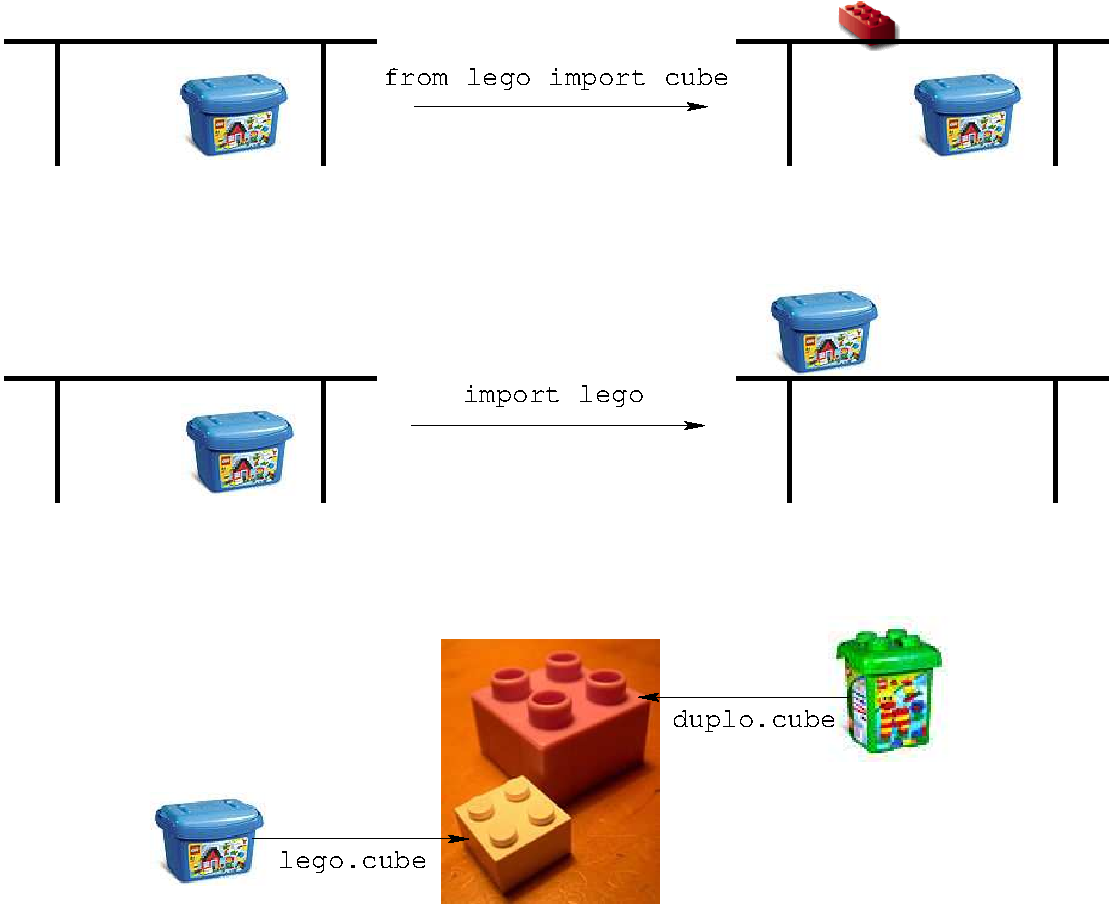
\includegraphics[width=8.75cm]{../fig/lego.pdf}$$

\end{frame}
\note{
\null\vfill

\begin{rem}
Les procédures et les fonctions intégrées au langage sont 
relativement peu nombreuses : ce sont seulement celles qui sont susceptibles 
d'être utilisées très fréquemment. 
Les autres fonctions sont regroupées dans des fichiers séparés que l'on appelle des modules.

Les modules sont donc des fichiers qui regroupent des ensembles de fonctions. 
Souvent on regroupe dans un même module des ensembles de fonctions 
apparentées que l'on appelle des bibliothèques.
Pour pouvoir utiliser ces fonctions, il faut importer le module correspondant.
$$\begin{py}{5cm}\tt
>>> from math import sin, pi\\
>>> sin(pi/2)\\
1.0
\end{py}
\hfill
\begin{py}{5cm}\tt
>>> import math\\
>>> math.sin(math.pi/2)\\
1.0
\end{py}$$
\end{rem}
}
%------------------------------------------



%------------------------------------------
\begin{frame}<presentation>
\frametitle{Définition d'une fonction}
%------------------------------------------
\begin{block}{Les 6 étapes de définition}
\begin{description}
\item[Nom:] un identificateur suffisamment explicite.
\pause
\item[Paramètres:] la liste des paramètres d'entrée-sortie de l'algorithme.
\pause
\item[Préconditions:] une liste d'expressions booléennes qui précisent les
	\alert{conditions d'application} de l'algorithme.
\pause
\item[Appel:] des exemples d'utilisation de l'algorithme avec les résultats
	attendus.
\pause
\item[Description:] une phrase qui dit \alert{ce que fait l'algorithme}.
\pause
\item[Code:] la séquence d'instructions nécessaires
	à la résolution du problème.
\end{description}
\end{block}

\end{frame}
\note{
\null\vfill

\begin{rem}
Pour encapsuler un algorithme dans une fonction, on suivra pas à pas 
la démarche suivante :
\begin{enumerate}
\item donner un nom explicite à l'algorithme,
\item définir les paramètres d'entrée-sortie de l'algorithme,
\item préciser les préconditions sur les paramètres d'entrée,
\item donner des exemples d'utilisation et les résultats attendus,
\item décrire par une phrase ce que fait l'algorithme et dans quelles conditions il le fait,
\item encapsuler l'algorithme dans la fonction spécifiée par les 5 points
	précédents.
\end{enumerate}
Les 5 premières étapes relèvent de la spécification de l'algorithme et la
dernière étape concerne l'encapsulation proprement dite de l'algorithme.
\end{rem}
}
%------------------------------------------



%------------------------------------------
\begin{frame}<presentation>
\frametitle{Nom et paramètres d'entrée-sortie}
%------------------------------------------
\begin{columns}[T]
\column{5.75cm}
\begin{enumerate}
\item<1-> {\em nom}\\
\begin{minipage}[t]{4.75cm}\scriptsize\tt
\mbox{}\alert{def} factorielle\alert{()}:\\
\mbox{}\ \ \ \ \alert{return}\\
\mbox{}
\end{minipage}

\item<2-> {\em paramètres d'entrée-sortie}\\
\begin{minipage}[t]{4.75cm}\scriptsize\tt
def factorielle(\alert{n}):\\
\mbox{}\ \ \ \ \alert{f = 1}\\
\mbox{}\ \ \ \ return \alert{f}
\end{minipage}

\end{enumerate} 

\column{5.75cm}
\begin{enumerate}
\item<1-> {\em nom}\\
\begin{minipage}[t]{4.75cm}\scriptsize\tt
>>> factorielle()\\
>>>\\
\mbox{}
\end{minipage}

\item<2-> {\em paramètres d'entrée-sortie}\\
\begin{minipage}[t]{4.75cm}\scriptsize\tt
>>> factorielle(5)\\
1\\
>>> factorielle(-5)\\
1\\
>>> factorielle('toto')\\
1
\end{minipage}

\end{enumerate} 
\end{columns}
\vspace*{5mm}

\pause

$$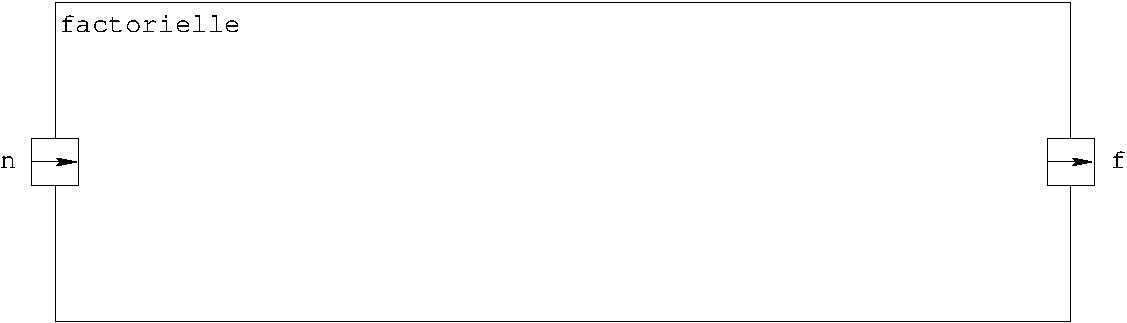
\includegraphics[width=7cm]{../fig/fact-2.pdf}$$

\end{frame}
\note{
{\bf Définitions}\begin{description}
\item[paramètres d'entrée] arguments de la fonction
	qui sont nécessaires pour effectuer le traitement associé
	à la fonction.
\item[paramètres de sortie] résultats retournés 
	par la fonction après avoir effectué le traitement associé
	à la fonction.
\end{description}
}
%------------------------------------------

%------------------------------------------
\begin{frame}<presentation>
\frametitle{Préconditions}
%------------------------------------------
\begin{columns}[T]
\column{5.75cm}
\begin{enumerate}\setcounter{enumi}{2}
\item {\em préconditions}
\begin{minipage}[t]{4.75cm}\scriptsize\tt
def factorielle(n)\\
\mbox{}\ \ \ \ \alert{assert type(n) is int}\\
\mbox{}\ \ \ \ \alert{assert n >= 0}\\
\mbox{}\ \ \ \ f = 1\\
\mbox{}\ \ \ \ return f
\end{minipage}
\end{enumerate} 

\column{5.75cm}
\begin{enumerate}\setcounter{enumi}{2}
\item {\em préconditions}
\begin{minipage}[t]{4.75cm}\scriptsize\tt
>>> factorielle(5)\\
1\\
>>> factorielle(-5)\\
{\color{red}AssertionError: \\
\mbox{}\ \ assert n >= 0}\\
>>> factorielle('toto')\\
{\color{red}AssertionError: \\
\mbox{}\ \ assert type(n) is int}\\
\end{minipage}
\end{enumerate} 
\end{columns}
\vspace*{5mm}

\pause
$$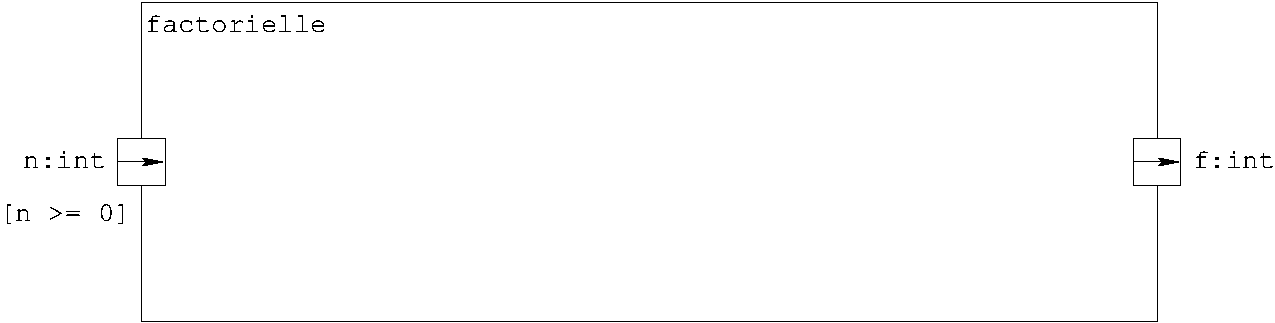
\includegraphics[width=7cm]{../fig/fact-3.pdf}$$
\end{frame}
\note{
{\bf Définitions}\begin{description}
\item[préconditions] conditions que doivent 
	impérativement vérifier les paramètres d'entrée 
	de la fonction juste avant son exécution.
\item[postconditions] conditions que doivent 
	impérativement vérifier les paramètres de sortie de la
	fonction juste après son exécution.
\item[invariants] conditions que doit impérativement 
	vérifier la fonction tout au long de son exécution.
\end{description}
}
%------------------------------------------


%------------------------------------------
\begin{frame}<presentation>
\frametitle{Jeu de tests}
%------------------------------------------
\begin{columns}[T]
\column{5.75cm}
\begin{enumerate}\setcounter{enumi}{3}
\item {\em jeu de tests}
\begin{minipage}[t]{5.5cm}\scriptsize\tt
def factorielle(n):\\
\mbox{}\ \ \ \ \alert{"""}\\
\mbox{}\ \ \ \ \alert{>>> for i in range(8):}\\
\mbox{}\ \ \ \ \alert{...\ \ \ \ \ print(factorielle(i),end=' ')}\\
\mbox{}\ \ \ \ \alert{1 1 2 6 24 120 720 5040}\\
\mbox{}\ \ \ \ \alert{"""}\\
\mbox{}\ \ \ \ assert type(n) is int\\
\mbox{}\ \ \ \ assert n >= 0\\
\mbox{}\ \ \ \ f = 1\\
\mbox{}\ \ \ \ return f
\end{minipage}
\end{enumerate}

\column{5.75cm}
\begin{enumerate}\setcounter{enumi}{3}
\item {\em jeu de tests}
\begin{minipage}[t]{5cm}\scriptsize\tt
>>> for i in range(8):\\
...\ \ \ \ \ print(factorielle(i),end=' ')\\
...\\
1 1 1 1 1 1 1 1
\end{minipage}
\end{enumerate} 

\end{columns}
\pause

\end{frame}
\note{
\null\vfill

\begin{rem}
A chaque étape de la spécification, le code de la fonction doit toujours être
exécutable même s'il ne donne pas encore le bon résultat.

Le jeu de tests ne sera vérifié
qu'une fois l'implémentation correctement définie.
\end{rem}

\begin{rem}[test automatique]
En \python, le jeu de tests peut être automatiquement
évalué par l'interpréteur en ajoutant les 3 lignes suivantes en fin de fichier source.
$$\begin{py}{6cm}\tt
if \_\_name\_\_ == "\_\_main\_\_" :\\
\mbox{}\ \ import doctest\\
\mbox{}\ \ doctest.testmod()
\end{py}$$
\end{rem}
}
%------------------------------------------

%------------------------------------------
\begin{frame}<presentation>
\frametitle{Description}
%------------------------------------------
\begin{columns}[T]
\column{5.75cm}
\begin{enumerate}\setcounter{enumi}{4}
\item {\em description}
\begin{minipage}[t]{5.5cm}\scriptsize\tt
def factorielle(n):\\
\mbox{}\ \ \ \ {"""}\\
\mbox{}\ \ \ \ \alert{f = n!}\\
\mbox{}\ \ \ \ {>>> for i in range(8):}\\
\mbox{}\ \ \ \ {...\ \ \ \ \ print(factorielle(i),end=' ')}\\
\mbox{}\ \ \ \ {1 1 2 6 24 120 720 5040}\\
\mbox{}\ \ \ \ {"""}\\
\mbox{}\ \ \ \ assert type(n) is int\\
\mbox{}\ \ \ \ assert n >= 0\\
\mbox{}\ \ \ \ f = 1\\
\mbox{}\ \ \ \ return f
\end{minipage}
\end{enumerate}

\column{5.75cm}
\begin{enumerate}\setcounter{enumi}{4}
\item {\em description}
\begin{minipage}[t]{5cm}\scriptsize\tt
>>> for i in range(8):\\
...\ \ \ \ \ print(factorielle(i),end=' ')\\
...\\
1 1 1 1 1 1 1 1
\end{minipage}
\end{enumerate} 

\end{columns}
\pause

\end{frame}
\note{
{\bf Définitions}\begin{description}
\item[description] phrase qui précise ce que fait la fonction 
	et dans quelles conditions elle le fait.
\end{description}
\null\vfill

\begin{rem}
La description est une  phrase (chaîne de caractères) qui doit
expliciter le rôle des paramètres d'entrée et leurs préconditions,
ainsi que toutes autres informations jugées nécessaires par le
concepteur de la fonction. 

Dans certains cas « difficiles », on pourra préciser une référence bibliographique ou un site {\sc Web}
où l'utilisateur pourra trouver des compléments sur la fonction et l'algorithme associé.

La description d'une fonction intègrera donc au moins :
\begin{itemize}
\item un exemple typique d'appel de la fonction,
\item la signification des paramètres d'entrée-sortie,
\item les préconditions sur les paramètres d'entrée,
\item un jeu de tests significatifs.
\end{itemize}
\end{rem}

}
%------------------------------------------

%------------------------------------------
\begin{frame}<presentation>
\frametitle{Implémentation}
%------------------------------------------
\begin{columns}[T]
\column{5.75cm}
\begin{enumerate}\setcounter{enumi}{5}
\item {\em implémentation}
\begin{minipage}[t]{5.5cm}\scriptsize\tt
def factorielle(n):\\
\mbox{}\ \ \ \ {"""}\\
\mbox{}\ \ \ \ {f = n!}\\
\mbox{}\ \ \ \ {>>> for i in range(8):}\\
\mbox{}\ \ \ \ {...\ \ \ \ \ print(factorielle(i),end=' ')}\\
\mbox{}\ \ \ \ {1 1 2 6 24 120 720 5040}\\
\mbox{}\ \ \ \ {"""}\\
\mbox{}\ \ \ \ assert type(n) is int\\
\mbox{}\ \ \ \ assert n >= 0\\
\mbox{}\ \ \ \ {f = 1}\\
\mbox{}\ \ \ \ \alert{for i in range(1,n+1):} \\
\mbox{}\ \ \ \ \ \ \ \ \alert{f = f * i}\\
\mbox{}\ \ \ \ return f
\end{minipage}
\end{enumerate}

\column{5.75cm}
\begin{enumerate}\setcounter{enumi}{5}
\item {\em implémentation}
\begin{minipage}[t]{5cm}\scriptsize\tt
>>> for i in range(8):\\
...\ \ \ \ \ print(factorielle(i),end=' ')\\
...\\
1 1 2 6 24 120 720 5040
\end{minipage}
\end{enumerate} 

\end{columns}
\pause

\end{frame}
\note{}
%------------------------------------------


%------------------------------------------
\begin{frame}<presentation>[containsverbatim]
\frametitle{{\tt factorielle(n)} : tout en un}
%------------------------------------------
\footnotesize
\begin{lstlisting}
def factorielle(n):
    """
    f = n!
    >>> for i in range(10):
    ...     print factorielle(i),
    1 1 2 6 24 120 720 5040 40320 362880
    >>> factorielle(15)
    1307674368000L
    """
    assert type(n) is int
    assert n >= 0

    f = 1
    for i in range(1,n+1): f = f * i

    return f
\end{lstlisting}

\end{frame}
\note{
\null\vfill

\begin{td}[Décodage base b $\rightarrow$ décimal]\label{td:decoder}
La valeur décimale d'un nombre entier
codé en base $b$ peut être obtenue par l'algorithme suivant :\\
{\tt \mbox{}\ \ \ \ }\begin{py}{7.5cm}\tt
>>> n = 0\\
>>> for i in range(len(code)):\\
... \mbox{}\ \ \ \ n = n + code[i]*b**(len(code)-1-i)\\
... \\
>>> 
\end{py}\\[1mm]
Spécifier une fonction qui encapsule cet algorithme.
\end{td}
}
%------------------------------------------


%------------------------------------------
\begin{frame}<presentation>[containsverbatim]
\frametitle{{\tt sommeArithmetique(n)} : tout en un}
%------------------------------------------
\footnotesize
\begin{lstlisting}
def sommeArithmetique(n):
    """
    somme s des n premiers entiers
    
    >>> for n in range(7):
    ...     print sommeArithmetique(n) == n*(n+1)/2,
    True True True True True True True
    """
    assert type(n) is int
    assert n >= 0
q = q + 1
    s = n*(n+1)/2
    
    return s
\end{lstlisting}

\end{frame}
\note{
\null\vfill

\begin{td}[Division entière]
Le calcul du quotient $q$ et du reste $r$ de la division 
entière $a\div b$ $(a = bq + r)$ peut être obtenu par l'algorithme suivant :\\
{\tt \mbox{}\ \ \ \ }\begin{py}{7.5cm}\tt
>>> q,r = 0,a\\
>>> while r >= b:\\
... \mbox{}\ \ \ \ q = q + 1\\
... \mbox{}\ \ \ \ r = r - b\\
... \\
>>> 
\end{py}\\[1mm]
Spécifier une fonction qui encapsule cet algorithme.
\end{td}
}
%------------------------------------------

%------------------------------------------
\begin{frame}<presentation>
\frametitle{Spécification et implémentation}
%------------------------------------------
\begin{block}{Spécification d'un algorithme\hfill Quoi ?}
La spécification décrit la fonction et l'utilisation d'un algorithme
(\alert{ce que fait l'algorithme}).

\pause
L'algorithme est vu comme une boîte noire dont on ne connaît pas le
fonctionnement interne.
\end{block}
\pause
\begin{block}{Implémentation d'un algorithme\hfill Comment ?}
L'implémentation décrit le fonctionnement interne de l'algorithme
(\alert{comment fait l'algorithme}).

\pause
L'implémentation précise l'enchaînement des instructions nécessaires
à la résolution du problème considéré.
\end{block}

\end{frame}
\note{
{\bf Définitions}\begin{description}
\item[spécification]
	décrit ce que fait l'algorithme 
	et dans quelles conditions il le fait.
\item[implémentation]
	décrit comment fait l'algorithme pour satisfaire sa
	spécification.
\end{description}
}
%------------------------------------------

%------------------------------------------
\begin{frame}<presentation>
\frametitle{Spécification et implémentation}
%------------------------------------------
\footnotesize
La spécification décrit la fonction et l'utilisation d'un algorithme
\null\vfill

\centerline{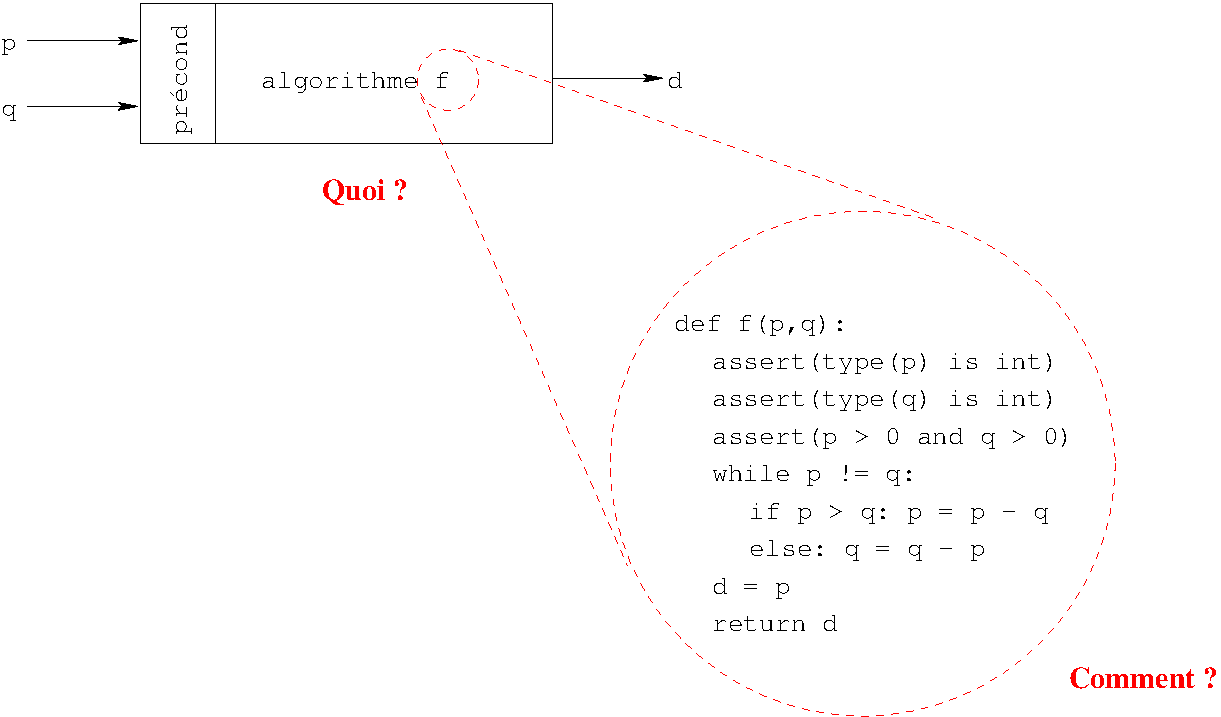
\includegraphics[width=8cm]{../fig/algo.pdf}}
\null\vfill 

\mbox{}\hfill L'implémentation décrit le fonctionnement interne de l'algorithme
\end{frame}\note{}
%------------------------------------------

%------------------------------------------
\begin{frame}<presentation>[containsverbatim]
\frametitle{Une spécification, des implémentations}
%------------------------------------------
\begin{columns}[T]\scriptsize
\column{5.75cm}
\begin{verbatim}
#--------------------------------------
def sommeArithmetique(n):
#--------------------------------------
    """
    somme s des n premiers entiers
    
    >>> for n in range(7):
    ...     print sommeArithmetique(n)\
                  == n*(n+1)/2
    True True True True True True True
    """
    assert type(n) is int
    assert n >= 0


    s = n*(n+1)/2
    
    return s
#--------------------------------------
\end{verbatim}

\column{5.75cm}
\begin{verbatim}
#--------------------------------------
def sommeArithmetique(n):
#--------------------------------------
    """
    somme s des n premiers entiers
    
    >>> for n in range(7):
    ...     print sommeArithmetique(n)\
                  == n*(n+1)/2
    True True True True True True True
    """
    assert type(n) is int
    assert n >= 0

    s = 0
    for i  in range(n+1): s = s + i
    
    return s
#--------------------------------------
\end{verbatim}
\end{columns}
\end{frame}
\note{
\null\vfill

\begin{td}[Une spécification, des implémentations]
\begin{enumerate}
\item Proposer deux implémentations du calcul de
la somme $s = \sum_0^n u_k$ des $n$ premiers termes d'une suite 
géométrique $u_k = a\cdot b^k$.
\item Comparer les complexités de ces deux im\-plé\-men\-ta\-tions.
\end{enumerate}

{\bf Indication:}
$$\displaystyle s = \sum_{k=0}^n ab^k = a\sum_{k=0}^n b^k$$

	où l'expression $\displaystyle N = (b^0+b^1+b^2+\cdots+b^n)$ peut être vue comme le nombre 
	$\displaystyle (111\cdots 1)_b$ en base $b$. Or en base $b$, le nombre $\displaystyle (b-1)(b^0+b^1+b^2+\cdots+b^n)$
	est le nombre immédiatement inférieur à $\displaystyle b^{n+1}$, soit $\displaystyle (b-1)N =
	b^{n+1}-1$.\\
	Exemple en base $b=10$ : $999_{10} = 9(10^0 + 10^1 + 10^2) = 10^3 - 1$
	$$\displaystyle S = \sum_{k=0}^n b^k = (b^0+b^1+b^2+\cdots+b^n) = \frac{b^{n+1}-1}{b-1}$$
\end{td}
}
%------------------------------------------

%------------------------------------------
\begin{frame}<presentation>
\frametitle{Concepteur versus Utilisateur}
%------------------------------------------
\begin{block}{Concepteur}
Le concepteur d'un algorithme définit l'interface et 
l'implémentation de l'algorithme.
\end{block}
\pause
\begin{block}{Utilisateur}
L'utilisateur d'un algorithme n'a pas à connaître son
implémentation; seule l'interface de l'algorithme le concerne.

\pause
Selon la spécification de l'algorithme,
l'utilisateur \alert{appelle} (utilise) l'algorithme sous forme d'une
\alert{procédure} ou d'une \alert{fonction}.
\end{block}

\end{frame}
\note{}
%------------------------------------------



%------------------------------------------
\begin{frame}<presentation>
\frametitle{Propriétés d'un algorithme}
%------------------------------------------
\begin{block}{Propriétés d'un algorithme}
\begin{description}
\item[validité :] être conforme aux jeux de tests
\pause
\item[robustesse :] vérifier les préconditions
\pause
\item[réutilisabilité :] être correctement paramétré
\end{description}
\end{block} 

\end{frame}
\note{
{\bf Définitions}\begin{description}
\item[Validité :] aptitude à réaliser 
	exactement la tâche pour laquelle il a été conçu.
	
	{\em ie}: L'implémentation de la fonction doit être conforme aux jeux de tests.
\item[Robustesse :] aptitude à se 
	protéger de conditions anormales d'utilisation.

	{\em ie}: La fonction doit vérifier impérativement ses préconditions.
\item[Réutilisabilité :] aptitude 
	à être réutilisé pour résoudre des tâches équivalentes à celle pour 
	laquelle il a été conçu.	

	{\em ie}: La fonction doit être correctement paramétrée.
\end{description}
\null\vfill

\begin{rem}
Une fois la fonction définie (spécifiée et implémentée), 
il reste à l'utiliser (à l'appeler).
\end{rem}
}
%------------------------------------------

%-------------------------------------------------------------------------
\end{document}
%-------------------------------------------------------------------------
